\documentclass[../main.tex]{subfiles}

\makeatletter
\@ifundefined{fromRoot}{%
  \newcommand{\fromRoot}[1]{../#1}
  
  \usepackage{xr}
  \externaldocument{../main}
}{}

\def\input@path{{\subfix{../}}}
%or: \def\input@path{{/path/to/folder/}{/path/to/other/folder/}}
\makeatother

\graphicspath{{\subfix{../}}}

\hypersetup{
    pdfauthor   = {TOURRES MAEL},
    pdftitle    = {Th\`{e}se (Chapitre 4)},
    pdfsubject  = {Th\`{e}se (Chapitre 4)},
%    pdfkeywords = {mots-cl\'{e}s},
}


\begin{document}

\selectlanguage{french}

\chapter{Extensions spécialisées avec 3 opérandes} 
\label{chapter:4}
\chaptermark{Extensions spécialisées avec 3 opérandes}

\etocsetnexttocdepth{4}
\etocsettocstyle{{\large \hspace{-1.5 em} \textbf{Contents} \hfill}\vspace{-2.5 em}\\\par\noindent\rule{\linewidth}{1 pt}\vspace{-.2 em}}{\par\noindent\rule{\linewidth}{1 pt}\\}
%
%
%
%
%
%
%
%
Ce chapitre étend les travaux présentés dans le chapitre précédent, utilisant  des opérations classiques à deux opérandes en entrées. 
Comme cela a été mentionné, ce choix, parfaitement valide au demeurant, reste la principale limitation bridant la conception d'instructions adaptées au décodage de CCE. 
Dans cette partie, nous évaluons les gains qu'il est possible d'atteindre en levant cette contrainte architecturale.
En effet, des cœurs RISC-V plus complexes permettent l'accès à 3 données pour exécuter, par exemple, des opérations de type MAC (Multiply And Accumulate). 
La première partie du chapitre expose les différentes caractéristiques architecturales de ces cœurs pouvant opérer sur trois registres d'entrée simultanément. 
Nous présentons également le cœur RISC-V sélectionné et la stratégie mise en œuvre pour insérer nos instructions dans l'ISA RISC-V.

Dans un second temps, nous présentons les différentes extensions mises au point et nous mettons en valeur les différences avec les résultats obtenus dans le chapitre précédent.
Pour terminer, une évaluation de l'impact de ces nouvelles extensions est réalisée. 
Les gains en termes de temps d'exécution sont exposés et mis en perspective des surcoûts matériels engendrés.
Ces expérimentations, comparables à celles réalisées pour les instructions à 2 registres, sont étendues pour les configurations SIMD sur 64 bits.


%
%
%
%
%
%
%
%
\localtableofcontents
%
%
%
%
%
%
%
%
\section{Modèle d'architecture ciblé}
%
%
%
%
%

Les cœurs de processeurs généralistes sont en principe conçus de manière à pouvoir délivrer 2 opérandes par cycle d'horloge à l'unité arithmétique et logique (UAL). 
Ce choix de conception est intrinsèquement lié à l'ISA des processeurs de type RISC où les instructions exécutées manipulent au plus 2 deux opérandes provenant des registres et/ou une valeur immédiate contenue dans un champ de l'instruction.
Cependant, certains cœurs de processeurs pensés pour exécuter plus efficacement des applications de traitement du signal possèdent un troisième port de lecture pour la file de registres, afin de permettre l'exécution d'instructions de type MAC (Multiply And Accumulate).
L'accès à une troisième opérande permet l'intégration d'opérations plus complexes au sein de l'UAL, dans le but de réduire le nombre d'instructions à réaliser, et par voie de conséquence, de diminuer le temps d'exécution des applicatifs ainsi que la taille de leur binaire.
Ces nouvelles opportunités ont toutefois un impact négatif sur la complexité matérielle de l'architecture, car elles nécessitent l'ajout d'un réseau de multiplexage supplémentaire dans la file de registres ou bien une duplication des bancs mémoire dans le but de délivrer cette donnée supplémentaire à l'UAL.
De plus, un format d'instruction supplémentaire doit être géré dans le décodeur d'instructions pour autoriser l'usage de cet troisième opérande.
L'augmentation de la complexité matérielle induite et le faible usage d'une troisième opérande dans l'UAL pour un bon nombre d'applications généralistes, limitent l'intégration de cette approche la majorité des cœurs RISC-V.


Dans le cadre de l'étude présentée dans les chapitres précédents, nous avons identifié et intégré des instructions possédant au maximum deux opérandes en entrée, notée dans ce chapitre \textbf{2R}.
Cette contrainte architecturale a limité certains choix de conception et n'a offert que peu d'opportunités pour exploiter au mieux les codes LDPC-NB et les turbo codes.
Dans ce chapitre, cette contrainte est allégée en considérant que l'UAL, et donc les instructions, sont en mesure de manipuler trois données/registres (\textit{rS1, rS2, rS3}).
La contrainte sur la sortie de l'UAL, elle reste inchangée, elle ne peut produire au maximum qu'une seule donnée (\textit{rD}).

Dans cette section, nous présentons une évolution des extensions conçues afin d'accélérer l'exécution des algorithmes de décodage des codes correcteurs d'erreurs.
L'utilisation d'une troisième opérande en entrée a nécessité une remise à plat des extensions proposées précédemment, pour aboutir à une solution efficace : certaines instructions à deux entrées ont été fusionnées, et d'autres ont aussi été créées et/ou modifiées afin de maintenir un flot d'exécution cohérent.

\textcolor{black}{Dans la spécification de base de l'ISA RISC-V, il n'existe pas de format standardisé permettant d'encoder directement 3 registres sources dans une instruction de type RV32/64I.
Afin de rester compatible avec cette ISA et ainsi de continuer à bénéficier des environnements de compilation, nous avons décidé d'utiliser le format proposé dans les extensions RV-FDQ (simple, double et quadruple précision en virgule flottante).
Ces dernières proposent un format 32 bits spécifique pour les opérations de type FMADD (Fused Multiplication-Accumulate) tel que cela est décrit dans le tableau \ref{R4_instruction}.}



%%%%%%%%%%%%%%%%%%%%%%%%%%%%
\begin{table}[]
    \centering
    \begin{tabular}{l|r}
        \toprule
         \textbf{Champ} & \textbf{Bits}  \\
         \bottomrule
         Opcode                 & [6:0]  \\
         Registre destination   & [11:7]  \\
         Fonction 3             & [14:12]  \\
         Registre source 1      & [19:15]  \\
         Registre source 2      & [24:20]  \\
         Fonction 2             & [26:25]  \\
         Registre source 3      & [31:27]  \\
        \bottomrule
    \end{tabular}
    \caption{Format 32 bits standardisé pour les instructions de type R4 (3 registres d'entrées) dans les spécifications RISC-V : RV-FDQ}
    \label{R4_instruction}
\end{table}
%%%%%%%%%%%%%%%%%%%%%%%%%%%%
Le détournement de ce format existant pour les opérations flottantes permet de réduire le surcoût matériel lié à l'introduction de nos extensions dans le décodeur d'instructions.
Afin de maintenir la compatibilité des cœurs avec l'extension F, nous avons sélectionné des \textit{opcodes} prévus pour l'ajout d'instructions spécialisées.
Ces derniers sont utilisés uniquement pour des instructions spécialisées additionnelles à deux ou trois opérandes et ont pour valeur $\times0b, \times3b, \times5b, \times7b$, conformément à la spécification RISC-V.
Il est à noter que les instructions manipulant seulement un ou deux registres utilisent comme précédemment le type R.

Les cœurs de RISC-V que nous avions auparavant sélectionnés possèdent des architectures internes simples et ne supportent pas par défaut les extensions F, D ou Q qui nécessitent une file de registres à 3 sorties pour exécuter les instructions de type FMA.
En conséquence, leurs décodeurs d'instructions n'étaient pas prévus pour décoder les instructions de type R et de générer les signaux de contrôle adéquats. En conséquence, pour éviter des temps d'ingénierie chronophages, nous avons décidé de changer de cible architecturale.
Parmi les cœurs RISC-V \textit{high-end} supportant ces extensions, nous pouvons citer par exemple les cœurs BOOM \cite{boom}, CVA6 \cite{zaruba2019cost}, SHAKTI \cite{shakti} et ROCKET \cite{rocket}.
Ces derniers, en plus de couvrir un nombre important d'extensions de l'ISA possèdent aussi un mode de fonctionnement 64 bits.

Les SoC dans lesquels ils sont intégrés possèdent des mémoires caches ainsi que bien d'autres périphériques leur permettant de faire démarrer un noyau Linux.
Pour des raisons techniques, nous avons sélectionné le cœur CVA6 développé par l'Open Hardware Group. 
Ce cœur, développé par ETH Zürich et poussé dans des projets étudiants par Thales, possède pour principal avantage d'être déployable sur les cartes de prototypage Digilent Genesys 2 que nous avions à disposition.


\begin{figure}
    \centering
    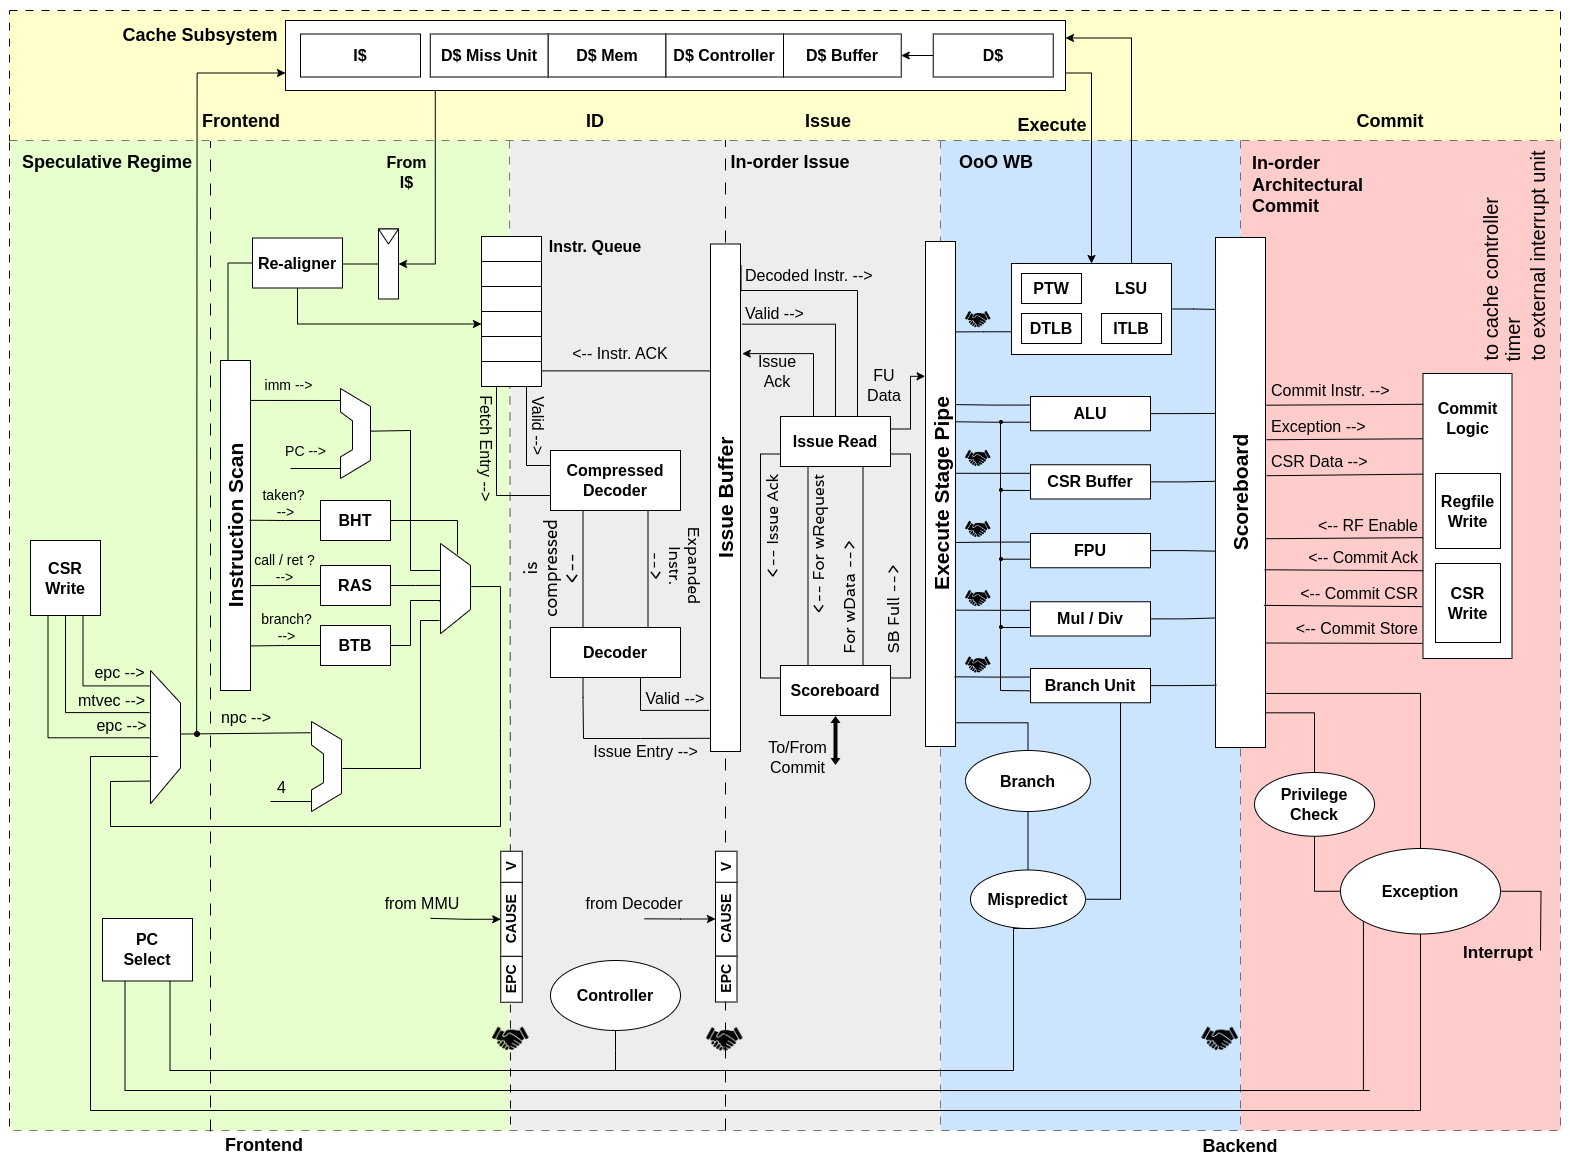
\includegraphics[scale=0.3]{chapter4/ariane_overview.drawio.png}
    \caption{Schéma de l'architecture du cœur CVA6.}
    \label{figure:cva6}
\end{figure}
%%%%%%%%%%%%%%%%%%%%%%%%%%%%%%%%%%%%%%%
%paragraphe 
%paragraphe 
\textcolor{black}{Le cœur CVA6 possède une architecture interne composée de 6 étages de pipeline, tel que cela est schématisé dans la figure \ref{figure:cva6}.
Il implante l'ISA de base RV64I, supporte nativement les extensions M/C/F et A de la spécification RISC-V et intègre un mécanisme de prédiction de branchement efficace. En interne, en fonction de la configuration du cœur, ce dernier peut opérer sur des données codées sur 32 bits ou 64 bits.
Ce dernier format de représentation des données, choisi avant la synthèse logique du cœur, permet d'appliquer un facteur de parallélisation deux fois supérieur lors des modes de fonctionnement SIMD. Toutefois, il est à noter que tout comme les cœurs RISC-V précédemment étudiés, le cœur CVA6 ne gère pas les accès mémoire aux données non-alignées. Les informations fournies dans le tableau \ref{tab:cva6:cost} permettent de quantifier la complexité du cœur CVA6 ainsi que du SoC dans lequel il est inclus. Les résultats présentés sont issus des rapports post-placement et routage pour un FPGA de type Xilinx Kintex 7 lorsqu'une fréquence de fonctionnement de 50 MHz est fixée.}
%%%%%%%%%%%%%%%%%%%%%%%%%%%%
\begin{table}[!tb]
    \centering
    \footnotesize
    \begin{tabular}{l|r|r|r|r|r|r}
    \toprule
        \textbf{Système}    & \textbf{CVA6} & \textbf{CVA6} & \textbf{CVA6} & \textbf{CVA6} & \textbf{CVA6} & \textbf{CVA6} \\
        \textbf{évalué}     & \textbf{cœur}& \textbf{cœur}& \textbf{cœur}& \textbf{SoC}  & \textbf{SoC}  & \textbf{SoC}  \\
    \midrule
        Chemin de données   & 64 bits       & 64 bits       & 64 bits       & 64 bits       & 64 bits       & 64 bits       \\
        Entrées dans l'UAL  & 2             & 3             & 3             & 2             & 3             & 3             \\ 
        ISA                 & RV64I         & RV64I         & RV64I         & RV64I         & RV64I         & RV64I         \\
        Extensions RV       & MAC           & MAC           & MACFD         & MAC           & MAC           & MACFD         \\
    \midrule
        LUT                 & 34576         & 34695         & 46615         & 59495         & 59624         & 71551         \\
        Flip-Flop           & 19806         & 19929         & 23954         & 41870         & 41993         & 46006         \\
        Blocs DSP           & 16            & 16            & 27            & 16            & 16            & 27            \\
        Blocs RAM           & 72            & 72            & 72            & 87            & 87            & 87            \\
    \bottomrule
    \end{tabular}
    \caption{Complexités matérielles des cœurs CVA6 avec SoC sur cible Kintex 7 lorsque 2 ou 3 opérandes sont accessibles dans l'UAL. Résultats post-placement routage avec fréquence de fonctionnement fixée à 50 MHz.}
    \label{tab:cva6:cost}
\end{table}
%%%%%%%%%%%%%%%%%%%%%%%%%%%%
%
%
%
%
\section{Évolution des extensions}
%
%
%
%
Dans cette partie, nous allons succinctement présenter les évolutions des extensions précédemment proposées.
Pour des raisons de lisibilité et de redondance, les descriptifs complets des instructions sont reportés en annexes.

L'utilisation de trois opérandes d'entrée permet de concevoir des instructions plus complexes en chaînant, par exemple, plus de ressources matérielles. 
Afin d'identifier les nouvelles instructions pour chaque famille de codes correcteurs d'erreurs, nous sommes repartis des spécifications algorithmiques et des listings assembleurs issus de nos descriptions logicielles initiales. 
Ceci, pour ne pas être influencé par des choix et des décisions issues de la première phase de nos travaux.

\textcolor{black}{Il résulte de cette analyse qu'en plus des instructions manipulant trois opérandes d'entrées, notées \textbf{3R}, il est nécessaire de conserver des instructions à une ou deux opérandes.
En effet, pour certaines opérations complexes qui pourraient être factorisées, certaines valeurs intermédiaires doivent aussi être stockées en mémoire pour une utilisation ultérieure. 
C'est le cas, par exemple, du calcul de la valeur absolue (\textit{i8\_abs\_pi8}), et des additions/soustractions saturées (\textit{i8\_add\_sat127\_pi8} et \textit{i8\_sub\_sat127\_pi8}). 
L'extension du jeu d'instructions que nous avons ainsi développé, est une combinaison entre un sous-ensemble des instructions précédemment identifiées et de nouvelles instructions. 
Les instructions nouvellement définies, ainsi que celles issues du travail présenté dans le chapitre 3 sont résumées pour les codes LDPC dans le tableau \ref{tab:compartif_ldpc}. 
Dans ce tableau, les colonnes notées \textbf{2R} font référence aux extensions proposées dans le chapitre précédent, tandis que les colonnes labellisées \textbf{3R} décrivent les extensions nécessaires ici (qu'elles possèdent 2 ou 3 opérandes).}


%%%%%%%%%%%%%%%%%%%%%%%%%%%%%%%%%%%%%%%%%%%%%%%%%%%%
\begin{table}
    \centering
    \footnotesize
    \begin{tabular}{l|l|c|c|c|c}
        \toprule
    &\multirow{3}{*}{\textbf{Mnémonique}} &\multicolumn{2}{c|}{\textbf{Mode}} & \multicolumn{2}{c}{\textbf{Mode SIMD}} \\
                                        & &\multicolumn{2}{c|}{\textbf{SISD}} & \multicolumn{2}{c}{\textbf{inter-trames}} \\
                                                &&\textbf{2R}& \textbf{3R}& \textbf{2R} & \textbf{3R} \\
        \cmidrule(l){1-6} 
        
        \textbf{Instr.} & i8\_abs\_pi8	            &\checkmark	    &\checkmark	&\checkmark	    &\checkmark \\ 
        \textbf{à 2 reg.} & i8\_add\_sat127\_pi8	&\checkmark	    &\checkmark	&\checkmark	    &\checkmark \\ 
                    &i8\_min\_pi8	                &\checkmark	    &\checkmark	&\checkmark	    &\checkmark \\ 
                    &i8\_sub\_sat127\_pi8	        &\checkmark	    &\checkmark	&\checkmark	    &\checkmark \\ 
                    &i8\_cmpeq\_pi8	                &\checkmark	    &	        &\checkmark	    &  \\ 
                    &i8\_invB\_Aneq1\_pi8	        &\checkmark	    &	        &\checkmark	    &  \\ 
                    &i8\_max\_pi8	                &\checkmark	    &	        &\checkmark	    &  \\ 
                    &i8\_xorA\_signB\_pi8	        &\checkmark	    &	        &\checkmark	    &  \\ 
                    &i8\_sign\_pi8		            &               &           &\checkmark	    &\checkmark \\ 
        \cmidrule(l){1-6}        

        \textbf{Instr} &i8\_invC\_xorA\_signB\_pi8  &	            &\checkmark	&	            &\checkmark \\ 
        \textbf{à 3 reg.} &i8\_minC\_maxAB\_pi8		&               &\checkmark	&	            &\checkmark \\ 
                    &i8\_blendC\_cmpeqAB\_pi8	    &               &\checkmark	&	            &\checkmark \\   

        \cmidrule(l){1-6}
        \multicolumn{2}{l|}{\textbf{Total (2R|3R)}} &8              &7(4|3)     & 9             &8(5|3)     \\
        \bottomrule
    \end{tabular}
    \caption{Instructions proposées pour l'accélération du décodage des codes LDPC en utilisant 2 ou 3 opérandes.}
\label{tab:compartif_ldpc}
\end{table}
%%%%%%%%%%%%%%%%%%%%%%%%%%%%%%%%%%%%%%%%%%%%%%%%%%%%
%paragraph
%paragraph
On observe pour les codes LDPC que trois nouvelles instructions à 3 registres ont été proposées pour le mode d'exécution scalaire. Ces dernières, décrites dans le tableau \ref{tab:instrus_ldpc_3reg}, sont utilisées de la manière suivante :

\begin{itemize}
\item \textit{i8\_invC\_xorA\_signB\_pi8}: Permet de simplifier le calcul de parité en couplant le calcul du signe du LLR et la mise à jour de la valeur de parité. 
\item \textit{i8\_minC\_maxAB\_pi8}: Réalise la mise à jour de la valeur du \textit{min2} de l'algorihtme Min-Sum en une seule instruction.
\item \textit{i8\_blendC\_cmpeqAB\_pi8}: Met en œuvre un masque logique pour sélectionner la valeur de \textit{min1} ou de \textit{min2} lors de la génération du LLR en sortie.
\end{itemize}
%%%%%%%%%%%%%%%%%%%%%%%%%%%%%%%%%%%%%%%%%%%%%%%%%%%%
\begin{table}[tb]
    \centering
    \footnotesize
    \begin{tabular}{l||ll}
    \hline
    \textbf{Instruction}& \textbf{Mnémonique}      &  \textbf{Implantation}                                     \\ 
    \hline               
    Maximum puis minium &i8\_minC\_maxAB\_pi8 rD,rS1,rS2,rS3          & rD\hspace{6mm}  := MIN8(MAX8(rS1,rS2),rS3)\\ 
    \\
    Calcul du minimum  &i8\_blendC\_cmpeqAB\_pi8 rD,rS1,rS2,rS3 & mask\hspace{2mm} := (rS1==rS2)?0xff:0x00     \\
    et mise à jour      &                                     & min\_t\         := rS1 \& \sim mask         \\
                        &                                     & min\_u          := rS3 \&      mask         \\
                        &                                     & rD\hspace{6mm}  := min\_t \textbar  min\_u        \\ 
    \\
    Génération du message   &i8\_invC\_xorA\_signB\_pi8 rD,rS1,rS2,rS3 & rD\hspace{6mm} := rS1 \land (rS2 \geqslant  0)?rS3: -rS3\\
    sortant du noeud de parité                             &&\\
    \hline
    \end{tabular}
    \caption{Spécification des nouvelles instructions à 3 opérandes pour le décodage des codes LDPC.}
    \label{tab:instrus_ldpc_3reg}
    \end{table}
%%%%%%%%%%%%%%%%%%%%%%%%%%%%%%%%%%%%%%%%%%%%%%%%%%%%
\textcolor{black}{La mise au point de ces trois instructions spécialisées pour le mode scalaire a permis de remplacer quatre instructions précédemment déployées (\textbf{2R}).
Il est à noter que ces instructions à 3 opérandes permettent aussi de supprimer l'usage d'instructions arithmétiques et logiques RV32I qui étaient mises en œuvre dans les cœurs de calcul\footnote{Ces dernières n'apparaissent pas dans le tableau}.
Pour les architectures SIMD inter-trames, les résultats obtenus sont similaires à ceux obtenus précédemment.}

Contrairement au cas des codes LDPC où les nouvelles instructions \textbf{3R} sont une combinaison des instructions précédemment identifiées, pour les codes polaires l'extension à 3 opérandes a aussi permis d'optimiser la fonction \textbf{G} dont l'équation est fournie dans le chapitre 3.
En effet, celle-ci ne pouvait être accélérée auparavant.
La possibilité d'utiliser 3 opérandes en entrée de l'UAL permet d'inclure l'ensemble des traitements à réaliser au sein d'une seule et unique instruction, tel que cela est indiqué dans le tableau \ref{tab:instrus_polar_3reg}.


%%%%%%%%%%%%%%%%%%%%%%%%%%%%%%%%%%%%%%%%%%%%%%%%%%%%
  \begin{table}[!tb]
    \centering
    \footnotesize
      \begin{tabular}{l || l l }
      \hline
        \textbf{Instruction} & \textbf{Mnémonique}              & \textbf{Implantation} \\ 
        \hline                   
        Fonction G de           &i8\_Gx\_pi8 rD,rS1,rS2,rS3     & Addsat := sat127{rS1 + rS2} \\
        l'arbre de décodage SC  &                               & Subsat := sat127{rS2 - rS1} \\
                                &                               & rD \hspace{6mm} :=(rS3 == 0) ? Addsat : Subsat   \\
        \hline
      \end{tabular}
    \caption{Spécification de l'instruction pour la fonction \textbf{G} pour le décodage des codes polaires.}
    \label{tab:instrus_polar_3reg}
    \end{table}
%%%%%%%%%%%%%%%%%%%%%%%%%%%%%%%%%%%%%%%%%%%%%%%%%%%%
L'analyse des données présentées dans le tableau \ref{tab:compartif_polaire} permet de noter que l'utilisation de cette nouvelle instruction permet de se passer des instructions \textit{i8\_setMask\_Aeq1\_pi8}, \textit{i8\_add\_sat127\_pi8} et \textit{i8\_sub\_sat127\_pi8} et ainsi de réduire le nombre de modifications à apporter au décodeur d'instructions.
Afin d'accélérer le décodage des codes polaires utilisant l'algorithme SC, seules $4$ instructions sont maintenant requises.
Cette diminution d'un facteur $1.5\times$ du nombre d'instructions spécialisées, par rapport à l'approche \textbf{2R} va permettre de réduire significativement le nombre d'instructions à exécuter.
Le tableau \ref{tab:compartif_polaire}, met en évidence que les instructions présentées afin d'améliorer les opérations d'élagage de leur côté, ne bénéficient pas de ce 3\up{ème} opérande. Ainsi, l'accélération de l'élagage est toujours supportée par $5$ instructions \textbf{2R}.
%%%%%%%%%%%%%%%%%%%%%%%%%%%%%%%%%%%%%%%%%%%%%%%%%%%%
\begin{table}
    \centering
    \footnotesize
    \begin{tabular}{l|l|c|c|c|c|c|c}
        \toprule
        &\multirow{3}{*}{\textbf{Mnémonique}}&\multicolumn{2}{c|}{\textbf{Mode}} & \multicolumn{2}{c|}{\textbf{Mode SIMD}} & \multicolumn{2}{c}{\textbf{Mode SIMD}}\\
        &&\multicolumn{2}{c|}{\textbf{SISD}} & \multicolumn{2}{c|}{\textbf{inter-trames}} & \multicolumn{2}{c}{\textbf{intra-trame}}\\
        &&\textbf{2R}& \textbf{3R}& \textbf{2R} & \textbf{3R} & \textbf{2R} & \textbf{3R}\\
        \cmidrule(l){1-8}

        \textbf{Instr.}  &i8\_setMask\_Aeq1\_pi8	        &       &   &   \checkmark   &    &  \checkmark &     \\ 
        \textbf{à 2 reg.}    &i8\_add\_sat127\_pi8	        &   \checkmark   &   &   \checkmark   &    &  \checkmark &     \\ 	
            &i8\_sub\_sat127\_pi8	        &   \checkmark   &   &   \checkmark   &    &  \checkmark &     \\ 
            &i8\_clrA\_Bneq0\_pi8	        &   \checkmark   & \checkmark &   \checkmark   &  \checkmark &  \checkmark & \checkmark   \\ 		
            &i8\_Rx\_pi8			        &   \checkmark   & \checkmark &   \checkmark   &  \checkmark &  \checkmark & \checkmark   \\ 	
            &i8\_Fx\_pi8			        &   \checkmark   & \checkmark &   \checkmark   &  \checkmark &  \checkmark & \checkmark   \\ 	
        \cmidrule(l){1-8} 		
        \textbf{Instr.}  &i8\_Gx\_pi8				    &       & \checkmark &       &  \checkmark &    & \checkmark   \\
        \textbf{à 3 reg.} & & & & & & &\\
        \cmidrule(l){1-8} 
        \multicolumn{2}{l|}{\textbf{Total (2R|3R)}} &6      &4(3|1)& 6  &4(3|1) &6    &4(3|1) \\ 
        \bottomrule

        \toprule
        \multicolumn{7}{l}{Extension pour l'algorithme Fast-SC(F-SC)} \\
        \cmidrule(l){1-8} 
        \textbf{Instr.}  &i16\_add\_accA\_loB\_pi8       &       &   &   \checkmark   & \checkmark  &    &     \\
        \textbf{à 2 reg.} & i16\_add\_accA\_hiB\_pi8       &       &   &   \checkmark   & \checkmark  &    &     \\
            &i8\_sign\_pi16                 &       &   &   \checkmark   & \checkmark  &    &     \\
            &i8\_Hxor\_pi8                  &       &   &       &    &  \checkmark &  \checkmark  \\ 
            &i8\_Hadd\_pi8                  &       &   &       &    &  \checkmark &  \checkmark  \\ 
        \cmidrule(l){1-8} 
        \multicolumn{2}{l|}{\textbf{Total (2R|3R)}}   &6      &4(3|1)   & 9     &7(6|1)   &9    &6(5|1) \\ 
        \bottomrule
    \end{tabular}
    \caption{Instructions proposées pour l'accélération du décodage des codes polaires (algorithmes SC et F-SC) en utilisant 2 ou 3 opérandes.}
\label{tab:compartif_polaire}
\end{table}
%%%%%%%%%%%%%%%%%%%%%%%%%%%%%%%%%%%%%%%%%%%%%%%%%%%%
En procédant à une analyse similaire à celle que nous venons de décrire, un nouveau jeu d'instruction est ainsi identifié et reporté dans le tableau \ref{tab:instrus_ldpcnb_3reg} pour la famille de code LDPC-NB.
Celle-ci consiste en l'assemblage de plusieurs instructions spécifiques proposées précédemment et de nouvelles.
%%%%%%%%%%%%%%%%%%%%%%%%%%%%%%%%%%%%%%%%%%%%%%%%%%%%
\begin{table}[!tb]
    \centering
    \footnotesize
    \begin{tabular}{l || l l }
    \hline
    \textbf{Instruction} & \textbf{Mnémonique}    & \textbf{Implantation} \\ 
    \hline               
    Minimum entre C et              &u8\_min\_addsat\_pu8        & rD := Min(Sat63(rS1+rS2), rS3)        \\ 
    addition saturée de A et B      && \\      
    Comparaison égale ou supérieure  &u8\_cmpge\_AndB\_lo8C\_pu8 & rD := (rS1 >= rS2)? rS3[7:0]:0x00   \\
    de A et B retourne les 8 LSB de C && \\
    \hline
    \end{tabular}
    \caption{Nouvelles instructions spécifiques pour les codes LDPC-NB avec 3 registres sources.}
    \label{tab:instrus_ldpcnb_3reg}
    \end{table}
%%%%%%%%%%%%%%%%%%%%%%%%%%%%%%%%%%%%%%%%%%%%%%%%%%%%

%%%%%%%%%%%%%%%%%%%%%%%%%%%%%%%%%%%%%%%%%%%%%%%%%%%%
\begin{table}
    \centering
    \footnotesize
    \begin{tabular}{l|l|c|c|c|c|c|c}
    \toprule
        &\multirow{3}{*}{\textbf{Mnémonique}}&\multicolumn{2}{c|}{\textbf{Mode}} & \multicolumn{2}{c|}{\textbf{Mode SIMD}} & \multicolumn{2}{c}{\textbf{Mode SIMD}}\\
        &&\multicolumn{2}{c|}{\textbf{SISD}} & \multicolumn{2}{c|}{\textbf{inter-trames}} & \multicolumn{2}{c}{\textbf{intra-trame}}\\
        &&\textbf{2R}& \textbf{3R}& \textbf{2R} & \textbf{3R} & \textbf{2R} & \textbf{3R}\\
        \cmidrule(l){1-8}
        
        \textbf{Instr.}  &u8\_addu\_sat64\_pu8	        &   \checkmark   & \checkmark &   \checkmark   &   \checkmark   &  \checkmark  & \checkmark   \\ 
        \textbf{à 2 reg.}    &u8\_minu\_pu8	                &   \checkmark   & \checkmark &   \checkmark   &   \checkmark   &  \checkmark  &     \\ 	
            &u8\_subu\_sat64\_pu8	        &   \checkmark   & \checkmark &   \checkmark   &   \checkmark   &  \checkmark  & \checkmark   \\ 
            &u8\_maxu\_pu8			        &       &   &   \checkmark   &   \checkmark   &     &     \\ 	
            &u8\_cmpge\_pu8			        &       &   &   \checkmark   &       &     &     \\ 	
            &u8\_hminu\_pu8				    &       &   &       &       &  \checkmark  & \checkmark   \\ 
            &u8\_Aandb\_lo8B\_pu8		    &       &   &   \checkmark   &       &     &     \\ 
            \cmidrule(l){1-8} 
        \textbf{Instr.}  &u8\_min\_addsat\_pu8	        &       & \checkmark &       &   \checkmark   &     & \checkmark   \\
        \textbf{à 3 reg.}    &u8\_cmpge\_AandB\_lo8C\_pu8	    &       &   &       &   \checkmark   &     &     \\ 		
            \cmidrule{1-8}
        \multicolumn{2}{l|}{\textbf{Total (2R|3R)}}   &3      &4(3|1)& 5  &6(4|2) &4    &4(3|1) \\
        \bottomrule
    \end{tabular}
    \caption{Instructions proposées pour l'accélération du décodage des codes LDPC-NB en utilisant 2 ou 3 opérandes.}
\label{tab:compartif_ldpcnb}
\end{table}
%%%%%%%%%%%%%%%%%%%%%%%%%%%%%%%%%%%%%%%%%%%%%%%%%%%%
\textcolor{black}{Toutefois, du fait de la complexité accrue de l'algorithme de décodage (en logiciel), il est difficile d'extraire des instructions spécifiques pertinentes et compatibles avec les contraintes voulues. 
En effet, le nombre d'accès mémoires et la gestion des pointeurs mémoire complexifient l'analyse du code.
Les instructions pertinentes identifiées sont les suivantes: 
\begin{itemize}
    \item \textit{u8\_min\_addsat\_pu8}: permet une concaténation des instructions d'additions saturées, puis génère le minimum entre ce résultat et la troisième entrée.
    \item \textit{u8\_cmpge\_AandB\_lo8C\_pu8}: effectue une comparaison entre A et B puis renvoie les 8 premiers bits de C ou bien 0 selon le résultat de la comparaison. 
\end{itemize}
Comme pour les codes LDPC, l'utilisation de ces nouvelles instructions vont théoriquement aboutir à une réduction du nombre total d'instructions exécutées dans l'algorithme.
Une différence importante entre les versions inter et intra-trame est l'utilisation d'un minimum horizontal.
Une majorité des instructions à 2 registres sources de notre extension sont conservées.
Les nouvelles instructions à 3 registres permettent, quand à elles, d'améliorer la latence dans la fonction de calcul des nœuds de parité, à l'aide de la fonction \textit{u8\_min\_addsat\_pu8}.
Enfin, l'instruction \textit{cmpge\_AandB\_lo8C\_pu8} permet de simplifier l'étape de recherche de l'index de la valeur minimale du vecteur de données inter-trames.\\ }



Enfin, en ce qui concerne les turbo codes, les résultats sont grandement améliorés grâce à l'utilisation d'une architecture \textbf{3R}.
En effet, cette famille de codes bénéficie grandement des instructions à 3 registres sources, comme montré dans \ref{tab:instrus_turbo_3reg}.
Par exemple, les calculs nécessaires au parcours d'un treillis LTE de l'algorithme BCJR font appel à des opérations utilisant 3 données.
Il s'agit de la concaténation d'opérations simples : addition, soustraction et maximum.
On retrouve ces nouvelles instructions dans la table ci-dessous \ref{tab:compartif_turbo}.


%%%%%%%%%%%%%%%%%%%%%%%%%%%%%%%%%%%%%%%%%%%%%%%%%%%%
\begin{table}
    \centering
    \footnotesize
    \begin{tabular}{l|l|c|c|c|c|c|c}
        \toprule
        &\multirow{3}{*}{\textbf{Mnémonique}}&\multicolumn{2}{c|}{\textbf{Mode}} & \multicolumn{2}{c|}{\textbf{Mode SIMD}} & \multicolumn{2}{c}{\textbf{Mode SIMD}}\\
        &&\multicolumn{2}{c|}{\textbf{SISD}} & \multicolumn{2}{c|}{\textbf{inter-trames}} & \multicolumn{2}{c}{\textbf{intra-trame}}\\
        &&\textbf{2R}& \textbf{3R}& \textbf{2R} & \textbf{3R} & \textbf{2R} & \textbf{3R}\\
        \cmidrule(l){1-8}
        \textbf{Instr.} &i8\_max\_pi8        & \checkmark  & \checkmark  & \checkmark  & \checkmark  & \checkmark  & \checkmark  \\
        \textbf{à 2 reg.} &i8\_scale\_pi8      & \checkmark  & \checkmark  & \checkmark  & \checkmark  &    &    \\
            &i8\_sign\_pi8       &    &    & \checkmark  & \checkmark  &    &    \\
            &i8\_add\_pi8        &    &    & \checkmark  & \checkmark  & \checkmark  & \checkmark  \\
            &i8\_sub\_pi8        &    &    & \checkmark  & \checkmark  & \checkmark  & \checkmark  \\
            &i8\_add\_srl1\_pi8     &    &    & \checkmark  & \checkmark  &    &    \\
            &i8\_srl1\_pi8        &    &    & \checkmark  & \checkmark  &    &    \\
            &i8\_shuffle\_pi8    &    &    &    &    & \checkmark  & \checkmark  \\
            &i8\_add\_div2\_pi8  &    &    &    &    & \checkmark  & \checkmark  \\
            &i8\_sub\_div2\_pi8  &    &    &    &    & \checkmark  & \checkmark  \\
            &i8\_sat\_sub\_pi8   &    &    &    &    & \checkmark  & \checkmark  \\
            &i8\_scale\_add\_pi8 &    &    &    &    & \checkmark  & \checkmark  \\
        \cmidrule(l){1-8} 
        \textbf{Instr.}  &i8\_accumax\_pi8    &    & \checkmark  &    & \checkmark  &    &   \\
        \textbf{à 3 reg.}&i8\_maxpm\_pi8      &    & \checkmark  &    & \checkmark  &    &\checkmark\\
            &i8\_accupp\_pi8     &    & \checkmark  &    & \checkmark  &    & \checkmark  \\
            &i8\_accump\_pi8     &    & \checkmark  &    & \checkmark  &    & \checkmark  \\
        \cmidrule{1-8}
        \multicolumn{2}{l|}{\textbf{Total (2R|3R)}} &2 &6(2|4)& 7  &11(7|4) &8  &11(8|3) \\ 
        \bottomrule
    \end{tabular}
    \caption{Instructions proposées pour l'accélération du décodage des turbo codes en utilisant 2 ou 3 opérandes.}
\label{tab:compartif_turbo}
\end{table}
%%%%%%%%%%%%%%%%%%%%%%%%%%%%%%%%%%%%%%%%%%%%%%%%%%%%
NOTA BENE : Les instructions \textit{i8\_add\_div2\_pi8}, \textit{i8\_sub\_div2\_pi8}, \textit{i8\_sat\_sub\_pi8} et \textit{i8\_scale\_add\_pi8} ne figurent pas dans les chapitres précédents.

En effet, celles-ci ont été identifiées après l'écriture de ces chapitres, et conservent le type \textbf{2R} (ou 2 registres sources).
Puisque leur application est totalement intégrée à ce chapitre, elles sont ainsi présentées ici.
%%%%%%%%%%%%%%%%%%%%%%%%%%%%%%%%%%%%%%%%%%%%%%%%%%%%
\begin{table}[tb]
    \centering
    \footnotesize
      \begin{tabular}{l || l l }
      \hline
        \textbf{Instruction} & \textbf{Mnémonique}    & \textbf{Implantation} \\ 
        \hline   
        Addition accumulée                  & i8\_accupp\_pi8 rD,rS1,rS2,rS3    & rD := rS1 + rS2 + rS3                \\
        Addition et soustraction accumulée  & i8\_accump\_pi8 rD,rS1,rS2,rS3    & rD := rS1 - rS2 + rS3                \\
        Maximum accumulée                   & i8\_accumax\_pi8 rD,rS1,rS2,rS3   & rD := MAX8(MAX8(rS1+rS2),rS3)      \\
        Maximum entre A+B et C-B            & i8\_maxpm\_pi8 rD,rS1,rS2,rS3     & rD := MAX8( rS1 + rS2 , rS3 - rS2 ) \\
        \hline
      \end{tabular}
    \caption{Nouvelle Instruction spécifique pour les turbo codes avec 3 registres sources.}
    \label{tab:instrus_turbo_3reg}
    \end{table}
%%%%%%%%%%%%%%%%%%%%%%%%%%%%%%%%%%%%%%%%%%%%%%%%%%%%
Il est important de noter la forte comptabilité entre les instructions \textbf{3R} pour les différents modes de parallélisation, ce qui permet de diminuer d'autant la complexité du jeu d'instructions dédié.
La latence finale est également optimisée grâce au nombre d'instructions spécialisées mises en œuvre.
La version scalaire SISD bénéficie de 2 instructions, tandis que les architectures \textbf{3R}, ont à disposition entre 6 et 11 instructions spécialisées.
Les résultats de leur implantation matérielle sont présentés dans les sections suivantes.
%
%
%
% 
%
\section{Impact des nouvelles extensions de l'ISA}
%
%
%
%
%
\textcolor{black}{Afin de mesurer l'impact de ces nouvelles extensions, plusieurs campagnes de tests ont été effectuées. 
Deux métriques ont été mesurées pour évaluer les performances de nos propositions :}

\begin{itemize}
    \item Le nombre de cycles d'horloges nécessaires pour exécuter les algorithmes de décodage.
    \item L'augmentation de la complexité matérielle du cœur CVA6 et l'impact sur sa fréquence de fonctionnement.
\end{itemize}

Ces évaluations ont été réalisées en sélectionnant la configuration de base du cœur CVA6 (RV64I).
L'évaluation du temps d'exécution des différents algorithmes de décodage a été obtenu par simulation. 
Celles-ci ont été réalisées avec l'aide de l'outil \textit{verilator} (version 4.110) qui, à partir de la description en SystemVerilog du cœur CVA6, permet de réaliser des simulations \textit{Bit Accurate} et \textit{Cycle Accurate}.
Cette stratégie, a été privilégiée pour éviter des temps de synthèse logique prohibitifs. 
En effet, il faut compter environ une heure pour réaliser une synthèse et le placement routage du SoC contenant le cœur CVA6.
%
%
%
% 
% 
% 
\subsection{Évaluation des extensions scalaires}
%
%
%
%
Cette section présente les résultats obtenus pour les décodeurs de CCE étudiés lorsqu'ils opèrent sur des données scalaires, i.e. sans parallélisation SIMD. Les instructions spécialisées traitent des données de 8 bits.
Le tableau \ref{tab:perfs_scalaire_3regs} présente une synthèse des résultats obtenus pour l'ensemble des algorithmes de décodage évalués. 
Les résultats rapportés ici sont homogènes : l'ensemble des travaux présentés dans les chapitres 4 et 5 ont été rejoués pour l'architecture CVA6.
Dans le tableau \ref{tab:perfs_scalaire_3regs}, sont indiqués les temps nécessaires à l'exécution des versions basiques des décodeurs (\ding{182}, Baseline), des versions étendues précédentes (\ding{183}, \textbf{ISA 2R}) et des versions présentées dans ce chapitre (\ding{184}, \textbf{ISA 3R}).
Dans ce tableau, sont aussi indiqués les gains relatifs entre les différentes versions (\ding{182}$\rightarrow$\ding{184}, \ding{183}$\rightarrow$\ding{184}) afin de simplifier l'analyse.
%%%%%%%%%%%%%%%%%%%%%%%%%%%%%%%%%%%%%%%%%%%%%%%%%%%%% 
\begin{table}[!tb]
    \footnotesize
    \centering
    \begin{tabular}{llrrrrr}
        \toprule
        &                                                       & \textbf{LDPC}	    & \multicolumn{2}{r}{\textbf{polaire}}   & \textbf{LDPC-NB}	 & \textbf{turbo}        \\
        &                                                       & OMS	    & SC	    & F-SC	        & MS	     & MLM  \\
        \cmidrule(l){1-7}
        \ding{182} Baseline                         & cycles    & $95955$	& $454637$  & $239292$          & $1715625$	 & $1585822$    \\
        \cmidrule(l){1-7}
        
        \ding{183} SISD ISA 2R	                    & cycles    & $66013$	& $271609$  & $125008$          & $1357945$	 & $938893$     \\
        \ding{184} SISD ISA 3R	                    & cycles    & $56514$	& $257901$  & $114207$          & $1086453$	 & $819757$     \\
        \cmidrule(l){1-7}
        Gain (\ding{182}$\rightarrow$\ding{184})    & cycles    & $39441$	& $196 736$ & $125085$          & $629172$	 & $766065$     \\
        Gain (\ding{182}$\rightarrow$\ding{184})    & (\%)	    & $41.1\%$	& $43.2\%$  & $52.2\%$          & $36.6\%$   & $48.3\%$     \\
        \cmidrule(l){2-7}
        Gain (\ding{183}$\rightarrow$\ding{184})    & cycles	& $9499$	& $13 708$  & $10801$           & $271492$	 & $119136$     \\
        Gain (\ding{183}$\rightarrow$\ding{184})    & (\%)      & $14.3\%$	& $5.0\%$   & $8.6\%$           & $19.9\%$	 & $12.6\%$     \\
        \cmidrule(l){1-7}
            Débit \ding{182}                       &Kbits/s     & $141$     &    $900$  & $1711$            & $7$       & $390$\\ 
            Débit \ding{183}                       &Kbits/s     & $206$     &   $1508$  & $3276$            &  $9$      & $659$\\
            Débit \ding{184}                       &Kbits/s     & $240$     &   $1588$  & $3586$            & $12$      & $755$\\
        \midrule
        Accélération\\
          \ding{182} $\rightarrow$ \ding{184}       &           & 1.7$\times$ & 1.8$\times$ & 2.1$\times$ &  1.6$\times$  & 1.9$\times$ \\
        \bottomrule
    \end{tabular}
    \caption{Comparaison des performances des cœurs usant d'instructions à 2 et 3 entrées, configuration 8 bits SISD avec une fréquence de fonctionnement de 50 MHz. }
    \label{tab:perfs_scalaire_3regs} 
\end{table}
%%%%%%%%%%%%%%%%%%%%%%%%%%%%%%%%%%%%%%%%%%%%%%%%%%%%% 

Si l'on s'intéresse tout d'abord aux décodeurs LDPC, on peut noter une réduction du nombre de cycles d'horloge d'environ  $14\%$ entre la version précédente (ISA \textbf{2R} \ding{183}) et la version actuelle (ISA \textbf{3R} \ding{184}). 
Ces gains sont liés aux instructions à $3$ opérandes d'entrée que nous avons développées.
Par rapport à la version d'origine du décodeur, les $7$ instructions spécialisées que nous avons ajoutées ont permis de réduire le temps d'exécution de $41\%$ sur le cœur CVA6.


Pour les codes polaires, les gains sont plus limités lorsque l'on considère l'algorithme de décodage SC. 
En effet, le passage de la version \ding{183} à \ding{184} n'engendre qu'une modeste réduction de $5\%$ du temps d'exécution. 
Cette dernière n'ajoute qu'une seule instruction depuis la version \ding{183} avec l'instruction \textit{i8\_Gx\_pi8} appliquant la fonction \textbf{G} de l'arbre de décodage.
Cela permet de s'affranchir de l'utilisation des instructions d'addition et soustraction saturées ainsi que de la sélection conditionnelle. 
Toutefois, lors de la compilation, le compilateur GCC introduit des instructions supplémentaires de conversions entre les formats int8\_t $\leftrightarrow$ int32\_t lors de l'utilisation de l'instruction \textbf{i8\_Gx\_i8} à 3 entrées.
La pénalité liée à l'ajout de ces instructions d'extension de signe des opérandes est moins présente pour le décodeur élaguant l'arbre de décodage (F-SC).
Ainsi, une réduction de $8.6\%$ est mesurée entre les versions \ding{183} et \ding{184}.
L'accélération atteint même $52.2\%$ lorsque l'on compare la version \ding{182} et \ding{184}.


Les facteurs d'accélérations mesurés pour le décodage des codes LDPC-NB sont plus importants.
En effet, entre les versions \ding{183} et \ding{184} l'accélération avoisine les $20\%$.
Ce facteur d'accélération est issu de l'utilisation de la nouvelle instruction \textit{u8\_min\_addsat\_pu8} qui est mise en œuvre à la fois dans la fonction de mise à jour des messages des nœuds de variables vers les nœuds de parités ainsi que dans le calcul des nœuds de parités.
Ce gain important s'explique par la faible accélération issue des instructions proposées dans \ding{183}.
L'accélération obtenue par rapport à la solution initiale \ding{182} est de $\approx 37\%$.

% turbo
\textcolor{black}{Enfin, si l'on concentre notre attention sur les turbo décodeurs, une amélioration de $48\%$ est obtenue par la configuration \ding{184} par rapport à la configuration initiale \ding{182}. 
Les $4$ instructions (ainsi que les instructions \textbf{2R}) ajoutées dans \ding{184} par rapport à la configuration \ding{183} ont permis une réduction supplémentaire de $\approx 12\%$.
Les gains obtenus sont limités à ces niveaux à cause des accès mémoire (\textit{load}, \textit{store} et arithmétique des pointeurs) qui deviennent prépondérants par rapport aux instructions arithmétiques.}

\textcolor{black}{Les dernières lignes du tableau \ref{tab:perfs_scalaire_3regs} présentent le débit normalisé des décodeurs, pour une fréquence de fonctionnement à 50 MHz. 
Cette fréquence est liée à l'implantation matérielle du cœur CVA6 sur le FPGA Kintex-7 présent sur la carte Digilent Genesys 2.
Il est à noter que les instructions ajoutées dans le cœur CVA6 n'ont pas d'impact sur la fréquence maximale de fonctionnement.
Les résultats présentés mettent en exergue que les configurations \ding{184} des décodeurs offrent des gains substantiels grâce aux instructions spécialisées proposées.}

Afin d'estimer le coût matériel associé à l'implantation des ces instructions dans le cœur testé, les UAL correspondant à chaque configuration sont isolées et comparées à la version de l'UAL standard du cœur.
Les surcoûts, exprimés en LUT, sont présentés dans la figure \ref{tikz:alu_sisd}.

%%%%%%%%%%%%%%%%%%%%%%%%%%%%%%%%%%%%%%%%%%%%%%%%%%%%%%
\begin{figure}
    \center
    \pgfplotsset{
        % width=8cm,
    %    height=0.3\textheight,
        grid=major,
        major grid style={dotted},
        symbolic x coords={LDPC,POLAIRE, PL-FSC, 
        LDPC-NB,TURBO},
        legend style={
           fill,
           at={(0.50,-0.2)},
           legend columns=2,
           legend cell align=left,
           anchor=north
        },
     }
    \begin{tikzpicture}
        \begin{axis}[
            ybar,%ytick pos=left,
            bar width=0.25cm,
            ymin=0, 
            width=.7\linewidth,
            height=7cm,
            % ymax=650,
            %ytick={0,100,200,300,400,500},
            %yticklabels={0,100,200,300,400,500},
            %ylabel style={align=center},
            ylabel={Surcoût en LUTs}, xtick=data, xtick pos=bottom,
            xticklabel style={
            inner sep=0pt,
            anchor=north east, 
            rotate=20,
            }
        ]
        \addplot [draw=Paired-1, fill=Paired-1!40, postaction={pattern color = black!80!Paired-1!70, pattern=north west  lines}]table [x=x, y expr=\thisrowno{1}] {chapter4/data_tikz_sisd.txt};
        \addlegendentry{2R - 8 bits}
    
        \addplot [draw=Paired-3, fill=Paired-3!40, postaction={pattern color = black!80!Paired-3!70, pattern=north east  lines}]table [x=x, y expr=\thisrowno{2}] {chapter4/data_tikz_sisd.txt};
        \addlegendentry{3R - 8 bits}
    
        \end{axis}
    \end{tikzpicture}
    \caption{Surcôut des instructions spécialisées SISD dans l'UAL du cœur CVA6.}
    \label{tikz:alu_sisd}
\end{figure}
%%%%%%%%%%%%%%%%%%%%%%%%%%%%%%%%%%%%%%%%%%%%%%%%%%%%%%
\textcolor{black}{La figure \ref{tikz:alu_sisd} présente ainsi les résultats obtenus. 
Pour les codes LDPC, la configuration \textbf{2R} implante 8 instructions, soit 1 instruction supplémentaire par rapport à la configuration \textbf{3R} avec 7 instructions. Toutefois, le coût varie de presque $50\%$ entre ces 2 versions. CE gain provient de la simplification du multiplexeur de sortie de l'UAL.
Dans le cas des codes polaires, les algorithmes SC et Fast-SC (F-SC) partagent les mêmes implantations d'instructions en matériel pour les configurations \textbf{2R} et \textbf{3R}, ainsi les résultats observés sont similaires. L'implantation de 4 (\textbf{3R}) au lieu de 6 instructions (\textbf{3R}), permet de réduire l'empreinte matérielle associée de $\approx 30\%$.
Cette observation est également valable avec les codes LDPC-NB.
Enfin, pour les turbo codes, 6 instructions sont implantées pour la configuration (\textbf{3R}), contre seulement 2 (\textbf{2R}). On constate ainsi que le coût matériel augmente fortement et est plus que doublé ($137\%$). 
Il est à noter que toutes ces instructions sont implantées sans conséquences sur la fréquence de fonctionnement du cœur.}



%%
%
%
%
%
%
\subsection{Évaluation des extensions SIMD inter-trames}
%
%
%
%

\textcolor{black}{Dans les expérimentations précédentes, nous nous sommes focalisés sur les décodeurs manipulant des données scalaires. Nous allons maintenant étudier l'impact de ces nouvelles extensions lors de l'exécution de décodeurs bénéficiant d'une parallélisation inter-trames. 
Le CVA6 étant un cœur 64 bits, nous avons décidé de tester deux formats de parallélisation SIMD : 32 et 64 bits. 
Le premier traite quatre informations codées sur 8 bits chacune (\textbf{int8\_t$\times$4}), tandis que le second étend ce traitement à 8 données (\textbf{int8\_t$\times$8}). 
Les résultats de ces expérimentations sont résumés dans le tableau \ref{tab:perfs_inter_3regs}.}



\textcolor{black}{
Si l'on s'intéresse dans un premier temps aux performances des décodeurs LDPC manipulant des données codées sur \textbf{int8\_t$\times$4}, on observe une réduction de 12\% lors du passage  \ding{183}$\rightarrow$\ding{184}.
Cette observation est cohérente par rapport aux résultats des expérimentations SISD (tableau \ref{tab:perfs_scalaire_3regs}).
Pour la version manipulant des données \textbf{int8\_t$\times$4}, le gain mesuré est plus faible avec $9.2\%$.
Ceci est causé par le temps d'entrelacement des données en amont et en aval de l'étape de décodage, qui consomme 2 fois plus de cycles d'horloge.
Toutefois, comme le nombre de données manipulées est 2 fois plus élevé, avec un nombre de cycles d'horloge à peu près équivalent, le débit final est ainsi doublé.
Concernant les autres codes correcteurs, lorsqu'ils manipulent des données codées sur 32 bits, on remarque que les gains liés au passage de \ding{183}$\rightarrow$\ding{184} sont plus importants que ceux relevés lors des expérimentations en SISD.
Ils varient de 20\% à 26\% en fonction des familles de code, montrant l'intérêt de ces extensions d'instructions.
Des gains moins marqués sont observés pour les décodeurs manipulant des données de type \textbf{int8\_t$\times$8}.
En effet, pour les données \textbf{int8\_t$\times$8}, GCC introduit fréquemment des instructions d'extension de signe (32 bits $\rightarrow$ 64 bits) qui sont inutiles dans nos cas d'usage.
Ces dernières impactent négativement le temps d'exécution des décodeurs.
L'utilisation de nos instructions à 3 opérandes en mode \textbf{int8\_t$\times$8} permet de supprimer des données temporaires, et donc une partie de ces extensions de signe associées, augmentant de facto le facteur d'accélération.}



%%%%%%%%%%%%%%%%%%%%%%%%%%%%%%%%%%%%%%%%%%%%%%%%%%%%%%%%%%%%
\begin{table}[!tb]
    \footnotesize
    \centering
    \begin{tabular}{lllrrrrrrr}
        \toprule
        \multicolumn{2}{l}{\textbf{inter-trames}}       &&  \textbf{LDPC}& \multicolumn{2}{r}{\textbf{polaire}}&\textbf{LDPC-NB}   & \textbf{turbo}        \\
        	                                            &&           & OMS	    & SC	    & F-SC            & MS	     & MLM  \\
        \midrule
        int8    &\ding{182} Baseline                    & cycles    & $95955$	& $454637$  & $239292$       & $1715625$ & $1585822$    \\
        \cmidrule(l){1-8}
        int8\_t$\times$4 
            &\ding{183} ISA 2R                          & cycles    & $61443$	& $373854$  & $215509$       & $1292853$ & $1051247$    \\
        (32 bits)    
            &\ding{184} ISA 3R                          & cycles    & $54027$	& $292678$  & $167095$       & $969990$ & $804471$     \\
        
            \cmidrule(l){2-8} 
            &Gain (\ding{182}$\rightarrow$\ding{184})   & cycles    &  $41928$	& $161959$  &  $72197$       & $745635$	 & $781351$     \\
            &Gain (\ding{182}$\rightarrow$\ding{184})   & (\%)      & $43.7\%$  & $35.6\%$  &  $30.2\%$      & $43.5\%$  & $49.2\%$       \\  
        
            \cmidrule(l){3-8}        
            &Gain (\ding{183}$\rightarrow$\ding{184})   & cycles    &  $7416$	& $81176$   &  $48414$       & $322863$ & $246 776$    \\
            &Gain (\ding{183}$\rightarrow$\ding{184})   & (\%)      & $12.0\%$  & $21.7\%$  &  $22.4\%$      & $25.0\%$  & $23.4\%$       \\
        
            \cmidrule(l){2-8}
            &Débit \ding{182}                           &Kbits/s    & $ 141$    & $ 900$    & $1711$         &  $7$      & $390$             \\ 
            &Débit \ding{183}                           &Kbits/s    & $ 885$    & $4382$    &  $7602$        & $39$      & $2356$            \\
            &Débit \ding{184}                           &Kbits/s    & $1006$    & $5598$    &  $9805$        &  $52$     &  $3078$          \\
        \midrule
    
        int8\_t$\times$8
                &\ding{185} ISA 2R                      & cycles    & $57898$   &  $388220$	& $243988$       & $1359186$ & $1207724$    \\
        (64 bits)   
                &\ding{186} ISA 3R                      & cycles    & $52546$	&  $335032$	& $213560$       & $1015731$ & $1035964$    \\
        \cmidrule(l){2-8}
        
        &Gain (\ding{182}$\rightarrow$\ding{186})       & cycles    & $43409$	& $119605$  & $25732$        & $699894$	 & $549858$     \\
        &Gain (\ding{182}$\rightarrow$\ding{186})       & (\%)      & $45.2\%$  & $26.3\%$  & $10.8\% $       & $40.8\%$ & $34.6\%$       \\  
        \cmidrule(l){3-8}  
        
        &Gain (\ding{183}$\rightarrow$\ding{186})       & cycles    &  $5352$	&  $53188$  & $30428$        &  $343455$ &  $171760$     \\
        &Gain (\ding{183}$\rightarrow$\ding{186})       & (\%)      & $9.2\%$   &  $13.7\%$ & $12.4\% $      & $25.7\%$ & $14.2\%$       \\
        \cmidrule(l){2-8}                                

        &Débit \ding{182}                               &Kbits/s    & $141$     & $900$     & $1711$         & $7$    & $390$            \\ 
        &Débit \ding{185}                               &Kbits/s    & $1879$    & $8440$    & $13430$        & $75$   & $4101$           \\
        &Débit \ding{186}                               &Kbits/s    & $2070$    & $9780$    & $15343$        & $100$   & $4781$           \\
        
        \midrule
        Accélération\\
        %\midrule
        & \ding{182} $\rightarrow$ \ding{184} & 32 bits                     & 7.1$\times$   & 6.2$\times$   &  5.7$\times$      &   7.1$\times$     &   7.9$\times$ \\
        & \ding{182} $\rightarrow$ \ding{186} & 64 bits                     & 14.6$\times$ & 10.9$\times$   &  9.0$\times$      &  13.5$\times$     &   12.2$\times$ \\
        & \ding{184} $\rightarrow$ \ding{186} & 32 $\rightarrow$ 64 bits    & 2.1$\times$  & 1.7$\times$    &  1.6$\times$      &   1.9$\times$     &   1.6$\times$        \\
        \bottomrule
        \end{tabular}
    \caption{Comparaison des performances des cœurs usant d'instructions à 2 et 3 entrées, configuration SIMD inter-trames avec une fréquence de fonctionnement fixée à 50 MHz.}
    \label{tab:perfs_inter_3regs}
\end{table}
%%%%%%%%%%%%%%%%%%%%%%%%%%%%%%%%%%%%%%%%%%%%%%%%%%%%%%

L'ajout des extensions 32 bits et 64 bits apporte des gains notables en termes d'accélération du temps de calcul.
Toutefois, l'implantation des opérateurs matériels au sein de l'UAL du cœur CVA6 engendre aussi une augmentation de la complexité matérielle.
La figure \ref{tikz:cost_simd_inter} présente le surcoût effectif de ces extensions (\textbf{3R}) lorsqu'elles sont insérées dans le cœur CVA6. Il est à noter que, comme précédemment, l'ajout de ces extensions en matériel n'a pas eu d'influence sur la fréquence de fonctionnement maximale du cœur après placement et routage par l'outil Vivado.

Si l'on s'intéresse dans un premier temps aux extensions proposées pour les décodeurs LDPC, on observe que les surcoûts matériels sont équivalents ($5\%$ supérieur) en mode \textbf{2R} et \textbf{3R}. 
De fait, même si plusieurs instructions \textbf{2R} ont été fusionnées pour produire des instructions \textbf{3R}, une instruction \textbf{2R} supplémentaire a été ajoutée. 
Le surcoût matériel pour les codes polaires est quant à lui plus faible (4\%) que celui de l'extension \textbf{2R}.
L'implantation des codes polaire avec l'algorithme FAST-SC mobilise 3 instructions supplémentaires en mode \textbf{2R} et \textbf{3R} afin d'accélérer les nœuds de l'arbre élagué. Cette différence permet un début d'explication pour la différence de coût $\approx 25\%$ observée en comparaison avec les codes polaires simples. Toutefois, il y a aussi une différence entre les 2 modes précédemment observés.
Pour les codes LDPC-NB et les turbo codes, l'ajout de $2$ et $4$ instructions respectivement dans l'extension \textbf{3R} ont engendré une augmentation respective de $\approx 2\%$ et $\approx 77\%$ du coût en LUT.

\textcolor{black}{Ces coûts matériels, qui peuvent sembler importants, sont dans un premier temps à mettre en perspective par rapport au coût matériel du cœur CVA6 (tableau \ref{tab:cva6:cost}) qui nécessite $34576$ LUT dans sa configuration 64 bits.
Ainsi, l'augmentation de la complexité du cœur est comprise entre $1\%$ et $3\%$ en fonction de l'extension considérée.
Ces surcoûts peuvent être considérés comme marginaux lorsqu'on les compare aux facteurs d'accélération de $9\times$ à $14\times$ obtenus (tableau \ref{tab:perfs_inter_3regs}).}


%%%%%%%%%%%%%%%%%%%%%%%%%%%%%%%%%%%%%%%%%%%%%%%%%%%%%%
\begin{figure}
    \center
    \pgfplotsset{
        % width=8cm,
    %    height=0.3\textheight,
        grid=major,
        major grid style={dotted},
        symbolic x coords={LDPC,SC, Fast-SC, 
        LDPC-NB,TURBO},
        legend style={
           fill,
           at={(0.50,-0.2)},
           legend columns=2,
           legend cell align=left,
           anchor=north
        },
     }
    \begin{tikzpicture}
        \begin{axis}[
            ybar,%ytick pos=left,
            bar width=0.25cm,
            ymin=0, 
            grid=major,
            width=.7\linewidth,
            height=7cm,
            % ymax=650,
            %ytick={0,100,200,300,400,500},
            %yticklabels={0,100,200,300,400,500},
            %ylabel style={align=center},
            ylabel={Surcoût en LUTs}, xtick=data, xtick pos=bottom,
            xticklabel style={
            inner sep=0pt,
            anchor=north east,
            rotate=20,
            }
        ]
        \addplot [draw=Paired-1, fill=Paired-1!40, postaction={pattern color = black!80!Paired-1!70, pattern=north west  lines}]table [x=x, y expr=\thisrowno{1}] {chapter4/data_tikz_inter.txt};
        \addlegendentry{2R - 32 bits}
     
        \addplot [draw=Paired-3, fill=Paired-3!40, postaction={pattern color = black!80!Paired-3!70, pattern=north east  lines}]table [x=x, y expr=\thisrowno{2}] {chapter4/data_tikz_inter.txt};
        \addlegendentry{3R - 32 bits}
     
        \addplot [draw=Paired-7, fill=Paired-7!40, postaction={pattern color = black!80!Paired-7!70, pattern=crosshatch  dots} ]table [x=x, y expr=\thisrowno{3}] {chapter4/data_tikz_inter.txt};
        \addlegendentry{2R - 64 bits}
     
        \addplot [draw=Paired-5, fill=Paired-5!40, postaction={pattern color = black!80!Paired-5!70, pattern=horizontal lines} ]table [x=x, y expr=\thisrowno{4}] {chapter4/data_tikz_inter.txt};
        \addlegendentry{3R - 64 bits}
        \end{axis}
    \end{tikzpicture}
    \caption{Surcoût matériel induit par les extensions nécessaires à la parallélisation inter-trames en configuration 32 bits et 64 bits.}
    \label{tikz:cost_simd_inter}
\end{figure}
%%%%%%%%%%%%%%%%%%%%%%%%%%%%%%%%%%%%%%%%%%%%%%%%%%%%%%
% 
% 
% 
\subsection{Évaluation des extensions SIMD intra-trame}
%
%
%
Cette dernière section est consacrée à l'étude des extensions proposées pour le second schéma de parallélisation SIMD. 
Une partie des instructions est commune avec celles mises en œuvre pour la parallélisation inter-trames. 
Toutefois, d'autres instructions impliquant des réductions horizontales ont été nécessaires. L'objectif de ce schéma est de réduire la latence de traitement des décodeurs. 
Pour y parvenir, il est nécessaire d'exploiter un parallélisme calculatoire variable et/ou plus faible car les descriptions algorithmiques, malgré le fait qu'elles soient plus complexes, sont moins favorables.

\textcolor{black}{Les performances temporelles des décodeurs ainsi optimisés à l'aide des extensions présentées dans ce chapitre sont exposées dans le tableau \ref{tab:perfs_intra_3regs}, à l'exception des décodeurs LDPC qui à cause de leur nécessité de réaliser des accès non alignés en mémoire n'ont pu être évalués.}

Les données issues du tableau \ref{tab:perfs_intra_3regs} comparent les performances obtenues par les nouvelles extensions à \textbf{3R} par rapport à celles du chapitre précédent.
Par observation, dans un premier temps au décodage des codes polaires et plus précisément au décodeur SC, on remarque que le schéma de parallélisation SIMD en 32 bits manipulant 4 données en parallèle permet de réduire de 76\% le temps d'exécution par rapport à l'approche naïve (\ding{182}, Baseline).
Par rapport à la version \textbf{2R}, l'utilisation de \textbf{3R} apporte un gain supplémentaire de 23\%.
Ces ordres de grandeur se retrouvent pour les expérimentations réalisées pour l'algorithme F-SC.

Les gains obtenus pour le décodage des turbo codes sont plus conséquents. Par rapport à la version naïve, le temps d'exécution de la version \textbf{3R} est réduit de 90\%.
Les nouvelles extensions mises au point grâce à la 3\up{ème} opérande ont permis de réduire de 45\% le temps d'exécution de la version \textbf{2R}.

\textcolor{black}{Les gains observés pour les décodeurs LDPC-NB atteignent $27\%$ et $27.1\%$ lorsque comparés au décodeur de base. Théoriquement, l'utilisation de 8 données concurrentes en parallèle (\textbf{int8\_t\times8}) devrait améliorer significativement la latence de décodage par rapport à 4 données (\textbf{int8\_t\times4}), contrairement à ce qui est observé.
Ces résultats sont principalement liés à l'inadéquation de la stratégie de parallélisation vis-à-vis des opérations mises en oeuvre dans l'algorithme de décodage, et du format des données par rapport à la largeur de l'unité SIMD.
En effet, le format $\mathbb{GF}$=16 nécessiterait des instructions SIMD sur 16\times8 bits pour accélérer les multiplications et les divisions dans $\mathbb{GF}$.}

Les facteurs d'accélération entre les versions originales des décodeurs et des implantations (\ding{182} $\rightarrow$ \ding{184}), présentés dans le tableau \ref{tab:perfs_intra_3regs} soulignent ici aussi l'intérêt des extensions proposées.


%%%%%%%%%%%%%%%%%%%%%%%%%%%%%%%%%%%%%%%%%%%%%%%%%%%%%%%%%%%%%
%tab:perfs_intra_3regs
\begin{table}[!tb]
    \footnotesize
    \centering
    \begin{tabular}{lll rrrr}
    \toprule
    \multicolumn{2}{l}{\textbf{intra-trame}}&&\multicolumn{2}{r}{\textbf{polaire}} & \textbf{LDPC-NB} & \textbf{turbo}\\
            &                                       &           & SC	        & F-SC    & MS	    & MLM  \\
    \cmidrule(l){1-7}
    int8    &\ding{182} Baseline                    & cycles    & $454637$      & $239292$  & $1715625$ & $1585822$     \\
    \cmidrule(l){1-7}
    int8\_t$\times$4     
            &\ding{183} ISA 2R                      & cycles    & $139961$      & $55 031$  & $1270968$ & $269167$      \\
    (32 bits) &\ding{184} ISA 3R                    & cycles    & $108701$      & $42 684$  & $927114$ & $148194$      \\
           \cmidrule(l){2-7}
            &Gain (\ding{182}$\rightarrow$\ding{184})& cycles    & $345936$      & $196608$  & $788511 $	& $1437628$     \\
            &Gain (\ding{182}$\rightarrow$\ding{184})& (\%)      & $76.0\%$      & $82.1\%$  & $46.0\% $	& $90.6\%$     \\
            \cmidrule(l){3-7}
            &Gain (\ding{183}$\rightarrow$\ding{184})& cycles    & $31260$       & $12 347$  & $343854 $	& $120 973$     \\
            &Gain (\ding{183}$\rightarrow$\ding{184})& (\%)      & $22.3\%$      & $22.4\%$  & $27.0\% $	& $44.9\%$     \\
            \cmidrule(l){2-7}
            &Débit \ding{182}                       &Kbits/s    &  $900$        & $1711$    &    $7   $ &  $390$      \\ 
            &Débit \ding{183}                       &Kbits/s    & $2926$        & $7443$    &  $10    $ & $2300$     \\
            &Débit \ding{184}                       &Kbits/s    & $3768$        & $9596$    & $14     $ & $4178$     \\
            \midrule
    int8\_t$\times$8    
            &\ding{185} ISA 2R                       & cycles    & $102298$      & $24172$   & $1264971$ & $139404$      \\
    (64 bits)        &\ding{186} ISA 3R              & cycles    & $80894$       & $20660$   & $921355 $ & $ 67483$      \\
            \cmidrule(l){2-7}
            &Gain (\ding{182}$\rightarrow$\ding{186})& cycles    &   $373743$    & $218632$  & $794270 $	& $1518339$     \\
            &Gain (\ding{182}$\rightarrow$\ding{186})& (\%)      &   $82.2\%$    & $91.3\%$  & $46.3\% $	& $95.7\%$     \\
            \cmidrule(l){3-7}
            &Gain (\ding{185}$\rightarrow$\ding{186})& cycles    &   $21404$     & $3512$    &  $343616$ & $71921$       \\
            &Gain (\ding{185}$\rightarrow$\ding{186})& (\%)      &   $20.9\%$    & $14.3\%$  & $27.1\%$  & $51.5\%$     \\
            \cmidrule(l){2-7}
            &Débit \ding{182}                       &Kbits/s    &    $900$      & $1711$    & $7$       & $390$      \\ 
            &Débit \ding{185}                       &Kbits/s    &   $4003$      & $16945$   & $10$      & $4441$     \\
            &Débit \ding{186}                       &Kbits/s    &   $5063$      & $19825$   & $14$      & $8175$     \\
            \midrule
        Accélération\\
        %\midrule
    & \ding{182} $\rightarrow$ \ding{184}   & 32 bits                   & 4.2$\times$   & 5.6$\times$   & 1.9$\times$   & 10.7$\times$  \\
    & \ding{182} $\rightarrow$ \ding{186}   & 64 bits                   & 5.6$\times$   & 11.6$\times$  & 1.9$\times$   & 23.7$\times$  \\
    & \ding{185} $\rightarrow$ \ding{186}   & 32 $\rightarrow$ 64 bits  & 1.3$\times$   & 2.1$\times$   & 1$\times$     & 2.2$\times$   \\
    \bottomrule
    
    \end{tabular}
    \caption{Comparaison des performances des cœurs usant d'instructions à 2 et 3 entrées, configuration SIMD intra-trame avec une fréquence de fonctionnement fixée à 50 MHz.}
    \label{tab:perfs_intra_3regs}
\end{table}
%%%%%%%%%%%%%%%%%%%%%%%%%%%%%%%%%%%%%%%%%%%%%%%%%%%%%%
\textcolor{black}{Lorsque l'on s'intéresse à l'extension de la taille des données manipulées par nos extensions SIMD de 32 bits à 64 bits on observe une accélération variant d'un facteur $1\times \rightarrow 2\times$. 
Des facteurs d'accélération de $\approx 2\times$ sont obtenus pour certains codes, tandis que pour d'autres les accélérations sont moins favorables, voir bien inférieures à celles obtenues dans le cas de la parallélisation inter-trames.
Cela s'explique par un parallélisme de calcul plus difficilement exploitable en mode intra-trame.
Par exemple, concernant le décodage SC des codes polaires, le parallélisme de calcul varie lors du décodage.
Ainsi, au niveau des feuilles de l'arbre, seules des opérations scalaires sont réalisées.
En effet, durant une partie du processus de décodage, le doublement des unités de calculs est sans conséquence, limitant de fait l'accélération globale.
Le facteur d'accélération du décodeur LDPC-NB est bien inférieur aux attentes.
En effet, les accès non réguliers à la mémoire lors des calculs des CNs induisent des pénalités qui annulent les gains liés à nos extensions.}

\textcolor{black}{L'impact des extensions proposées pour l'accélération des décodeurs intra-trame sur la complexité matérielle a aussi été évaluée.
La figure \ref{tikz:cost:simd:intra} présente le surcoût des extensions en termes de LUT issues des rapports post-placement et routage.
Contrairement aux expérimentations réalisées en mode inter-trames, on peut observer une plus grande disparité entre les surcoûts des extensions \textbf{2R} et \textbf{3R}. 
Cela est lié au fait que la possibilité d'utiliser $3$ opérandes a permis de concevoir plus d'instructions spécialisées. 
C'est particulièrement le cas, par exemple, pour les turbo codes où l'utilisation d'une troisième opérande a permis de créer 4 instructions spécialisées supplémentaires.
Cela explique le doublement du coût de l'extension \textbf{3R} par rapport à l'extension \textbf{2R}.
Toutefois, même si cette observation devrait également se vérifier en mode 64 bits, l'outil Vivado réalise des optimisations durant les étapes post-placement et routage qui tempèrent cette tendance.
Un phénomène équivalent est observé pour l'extension dédiée aux code LDPC-NB où l'extension \textbf{2R} est plus onéreuse que la version \textbf{3R} en configuration 32 bits.
Enfin, si l'on compare le surcoût des extensions dédiées au mode intra-trame, par rapport à celles pour le mode inter-trames, on note qu'il est du même ordre de grandeur, à l'exception des instructions pour les turbo codes; ces dernières sont environ 20\% plus onéreuses. 
Comme nous l'avons précédemment évoqué, ces coûts matériels qui peuvent sembler importants ne représentent que de $1\%$ à $3\%$ de la complexité du CVA6.}



%%%%%%%%%%%%%%%%%%%%%%%%%%%%%%%%%%%%%%%%%%%%%%%%%%%%%%
\begin{figure}[!tb]
    \center
    \pgfplotsset{
        % width=8cm,
    %    height=0.3\textheight,
        grid=major,
        major grid style={dotted},
        symbolic x coords={SC, Fast-SC, LDPC-NB, TURBO},
        legend style={
           fill,
           at={(0.50,-0.2)},
           legend columns=2,
           legend cell align=left,
           anchor=north
        },
     }
    \begin{tikzpicture}
        \begin{axis}[
            ybar,%ytick pos=left,
            bar width=0.25cm,
            ymin=0, 
            width=.7\linewidth,
            height=7cm,
            % ymax=650,
            %ytick={0,100,200,300,400,500},
            %yticklabels={0,100,200,300,400,500},
            %ylabel style={align=center},
            ylabel={Surcoût en LUTs}, xtick=data, xtick pos=bottom,
            xticklabel style={
            inner sep=0pt,
            anchor=north east,
            rotate=20,
            }
        ]
        \addplot [draw=Paired-1, fill=Paired-1!40, postaction={pattern color = black!80!Paired-1!70, pattern=north west  lines}]table [x=x, y expr=\thisrowno{1}] {chapter4/data_tikz_intra.txt};
        \addlegendentry{2R - 32 bits}
     
        \addplot [draw=Paired-3, fill=Paired-3!40, postaction={pattern color = black!80!Paired-3!70, pattern=north east  lines}]table [x=x, y expr=\thisrowno{2}] {chapter4/data_tikz_intra.txt};
        \addlegendentry{3R - 32 bits}
     
        \addplot [draw=Paired-7, fill=Paired-7!40, postaction={pattern color = black!80!Paired-7!70, pattern=crosshatch  dots} ]table [x=x, y expr=\thisrowno{3}] {chapter4/data_tikz_intra.txt};
        \addlegendentry{2R - 64 bits}
     
        \addplot [draw=Paired-5, fill=Paired-5!40, postaction={pattern color = black!80!Paired-5!70, pattern=horizontal lines} ]table [x=x, y expr=\thisrowno{4}] {chapter4/data_tikz_intra.txt};
        \addlegendentry{3R - 64 bits}
        
    
        \end{axis}
    \end{tikzpicture}
    \caption{Surcoût matériel induit par les extensions nécessaires à la parallélisation intra-trame en configuration 32 bits et 64 bits.}
    \label{tikz:cost:simd:intra}
\end{figure}
%%%%%%%%%%%%%%%%%%%%%%%%%%%%%%%%%%%%%%%%%%%%%%%%%%%%%%

%
%
%
%
\section{Conclusion}
%
%
%
%
\textcolor{black}{Dans ce chapitre, nous avons présenté de nouvelles extensions permettant d'accélérer les algorithmes de décodage des CCE. 
Contrairement aux précédentes extensions, ces dernières bénéficient d'un accès possible à un troisième opérande. 
Cette opportunité a permis de proposer de nouvelles instructions en vue de minimiser le temps d'exécution des algorithmes. 
Les différentes extensions ont été déclinées sous plusieurs formes afin de permettre d'évaluer à la fois un traitement scalaire, et SIMD, des données. 
De plus, grâce à l'utilisation d'un cœur RISC-V plus complexe possédant un chemin de données 64 bits, nous avons pu étudier les options de passage à l'échelle des extensions proposées.}

\textcolor{black}{Le tableau \ref{tab:sum} propose une synthèse des facteurs d'accélération qui ont été mesurés pour les schémas de parallélisation SIMD. 
Les facteurs d'accélérations qui sont rapportés ont été calculés par rapport aux codes logiciels n'exploitant que le jeu d'instructions de base des cœurs RISC-V. 
Comme le met en évidence ce tableau, l'ensemble des extensions proposées offre des facteurs d'accélération élevés tandis que le nombre d'instructions ajouté à l'ISA est relativement faible. 
Par exemple, pour les codes polaires, le passage de $3$ opérandes d'entrées à permis de concevoir $1$ instruction qui permet d'atteindre une accélération avoisinant 10.7$\times$ (64 bits, mode inter-trames). 
Des facteurs d'accélération plus important ont été obtenus pour le décodage des turbo codes ($23.5\times$) au prix d'un nombre d'instructions spécialisées supérieur ($11$ instructions en mode 64 bits pour une parallélisation intra-trame). 
L'utilisation d'un troisième opérande d'entrée pour les opérations spécialisées a permis, en moyenne, d'augmenter le facteur d'accélération de $1.32\times$ (32\%) par rapport aux extensions \textbf{2R}.
Le choix de la stratégie de parallélisation impacte fortement sur les niveaux de performance atteignables. 
En effet, alors que la stratégie intra-trame permet d'atteindre un facteur d'accélération de $25.5\times$ pour les turbo codes, elle ne permet d'obtenir que $1.7\times$ pour le décodage des codes LDPC-NB où l'approche inter-trames offre $13.5\times$.}

\textcolor{black}{D'un point de vue matériel, les extensions \textbf{3R} ont des complexités matérielles comparables aux extensions \textbf{2R}.
En effet, le coût lié à l'ajout de nouvelles instructions est en partie compensée par les gains réalisés par la fusion d'autres instructions.
La fusion d'instructions engendrant par exemple une réduction du coût du multiplexeur sélectionnant les résultats en sortie de l'UAL.
Les résultats basés sur l'utilisation du cœur CVA6, obtenus post-placement routage, mettent en évidence le faible impact des extensions sur le coût global du cœur.
En effet, ces dernières induisent une augmentation limitée de 1\% à 3\% du coût du cœur en termes de LUT. 
Enfin, pour toutes les expérimentations que nous avons réalisées, aucune pénalité concernant la fréquence maximale de fonctionnement du cœur n'a été observée.}



%%%%%%%%%%%%%%%%%%%%%%%%%%%%%%%%%%%%
\begin{table}[!tb]
    \footnotesize
    \centering
    \begin{tabular}{llrrrrr}
    \toprule                    %2              % 3             % 4             % 5 
    \textbf{CCE}     &       & \textbf{2R}  & \textbf{3R}  & \textbf{2R}  & \textbf{3R}      \\
    \textbf{SIMD}   &       & \textbf{int8\_t$\times$4} & \textbf{int8\_t$\times$4} & \textbf{int8\_t$\times$8} & \textbf{int8\_t$\times$8} \\
        \textbf{Bits}    &       & \textbf{32}& \textbf{32} & \textbf{64} & \textbf{64} \\
        \cmidrule(l){1-6}
        LDPC    & inter-trames  & 885 Kbps  &1006 Kbps  & 1879 Kbps & 2070 Kbps \\
        OMS     &               & (\textcolor{black}{\textbf{6.2}}$\times$)  & (7.1$\times$)  &             (\textcolor{black}{\textbf{13.2}}$\times$) & (14.6$\times$) \\
        \cmidrule(l){1-6} 
        polaire      & inter-trames  & 4382 Kbps     &5506 Kbps      & 8440 Kbps     & 9633 Kbps     \\
        SC      &               & (4.9$\times$)   & (6.2$\times$)   & (9.4$\times$)   & (10.8$\times$)  \\
                & intra-trame   & 2926 Kbps     & 3768 Kbps     & 4003 Kbps     & 5063 Kbps     \\
                &               & (3.2$\times$)   & (4.2$\times$)   & (4.4$\times$)   & (5.6$\times$)   \\
        \cmidrule(l){1-6}
        polaire      & inter-trames  &7602 Kbps      &9625 Kbps      & 13430 Kbps    & 15212 Kbps    \\
        Fast-SC     &               & (4.4$\times$)   & (5.7$\times$)   & (7.8$\times$)   & (9$\times$)   \\
                & intra-trame   & 7443 Kbps     & 9596 Kbps     & 16495 Kbps    & 19825 Kbps    \\
                &               & (4.3$\times$)   & (5.6$\times$)   & (9.9$\times$)   & (11.6$\times$)  \\
        \cmidrule(l){1-6} 
        LDPC NB & inter-trames  & 39 Kbps       & 50  Kbps      & 75 Kbps       & 94 Kbps       \\
        MS      &               & (5.3$\times$)   & (7.0$\times$)   & (10.1$\times$)  & (13.5$\times$)  \\
                & intra-trame   & 10  Kbps      & 13 Kbps       & 10 Kbps       & 14 Kbps       \\
                &               & (1.3$\times$)   & (1.8$\times$)   & (1.3$\times$)   & (1.8$\times$)    \\
        \cmidrule(l){1-6} 
        TURBO   & inter-trames  & 2356 Kbps     &3078 Kbps      & 4101 Kbps     & 4781 Kbps     \\
        MLM     &               & (6.0$\times$)   &( 7.9$\times$)   & (10.5$\times$ ) & (12.2$\times$)   \\
                & intra-trame   & 2300 Kbps     & 4178 Kbps     & 4441 Kbps     & 8175 Kbps     \\
                &               & (5.9$\times$)   & (\textcolor{black}{\textbf{10.7}}$\times$)  & (11.4$\times$)  & (\textcolor{black}{\textbf{23.5$\times$}})   \\
        \bottomrule
    \end{tabular}
    \caption{Accélération observé des débits par rapport à la Baseline.}
    \label{tab:sum}
\end{table}
%%%%%%%%%%%%%%%%%%%%%%%%%%%%%%%%%%%%

\end{document}
